\chapter{Bakteri dan Ketahanan terhadap Antibiotik}\label{ch:g11:antibiotic-resistance}

Pada 1941 seorang polisi yang sedang sekarat karena keracunan darah
akibat sebuah goresan diberi dosis penisilin yang pertama kali dipakai
pada seorang pasien. Ia pulih dalam beberapa hari --- lalu kambuh dan
meninggal ketika persediaannya, yang disari susah payah dari kapang,
habis. Dalam sepuluh tahun penisilin dibuat berton-ton dan infeksi yang
telah membunuh selama ribuan tahun menjadi dapat disembuhkan dalam
sepekan. Dalam dua puluh tahun, bakteri yang tidak lagi tersentuh
penisilin menjadi lazim di tiap rumah sakit. Bab ini membahas
mengapa: bagaimana bakteri beragam, bagaimana sebuah \omterm{def:g11:antibiotic-resistance:antibiotic}{antibiotik}
memilahnya, dan bagaimana hitungan sebuah populasi bermiliar-miliar
mengubah \omterm{def:g11:mutations:mutation}{mutasi} yang langka menjadi persoalan sebangsal.

\begin{omfigure}
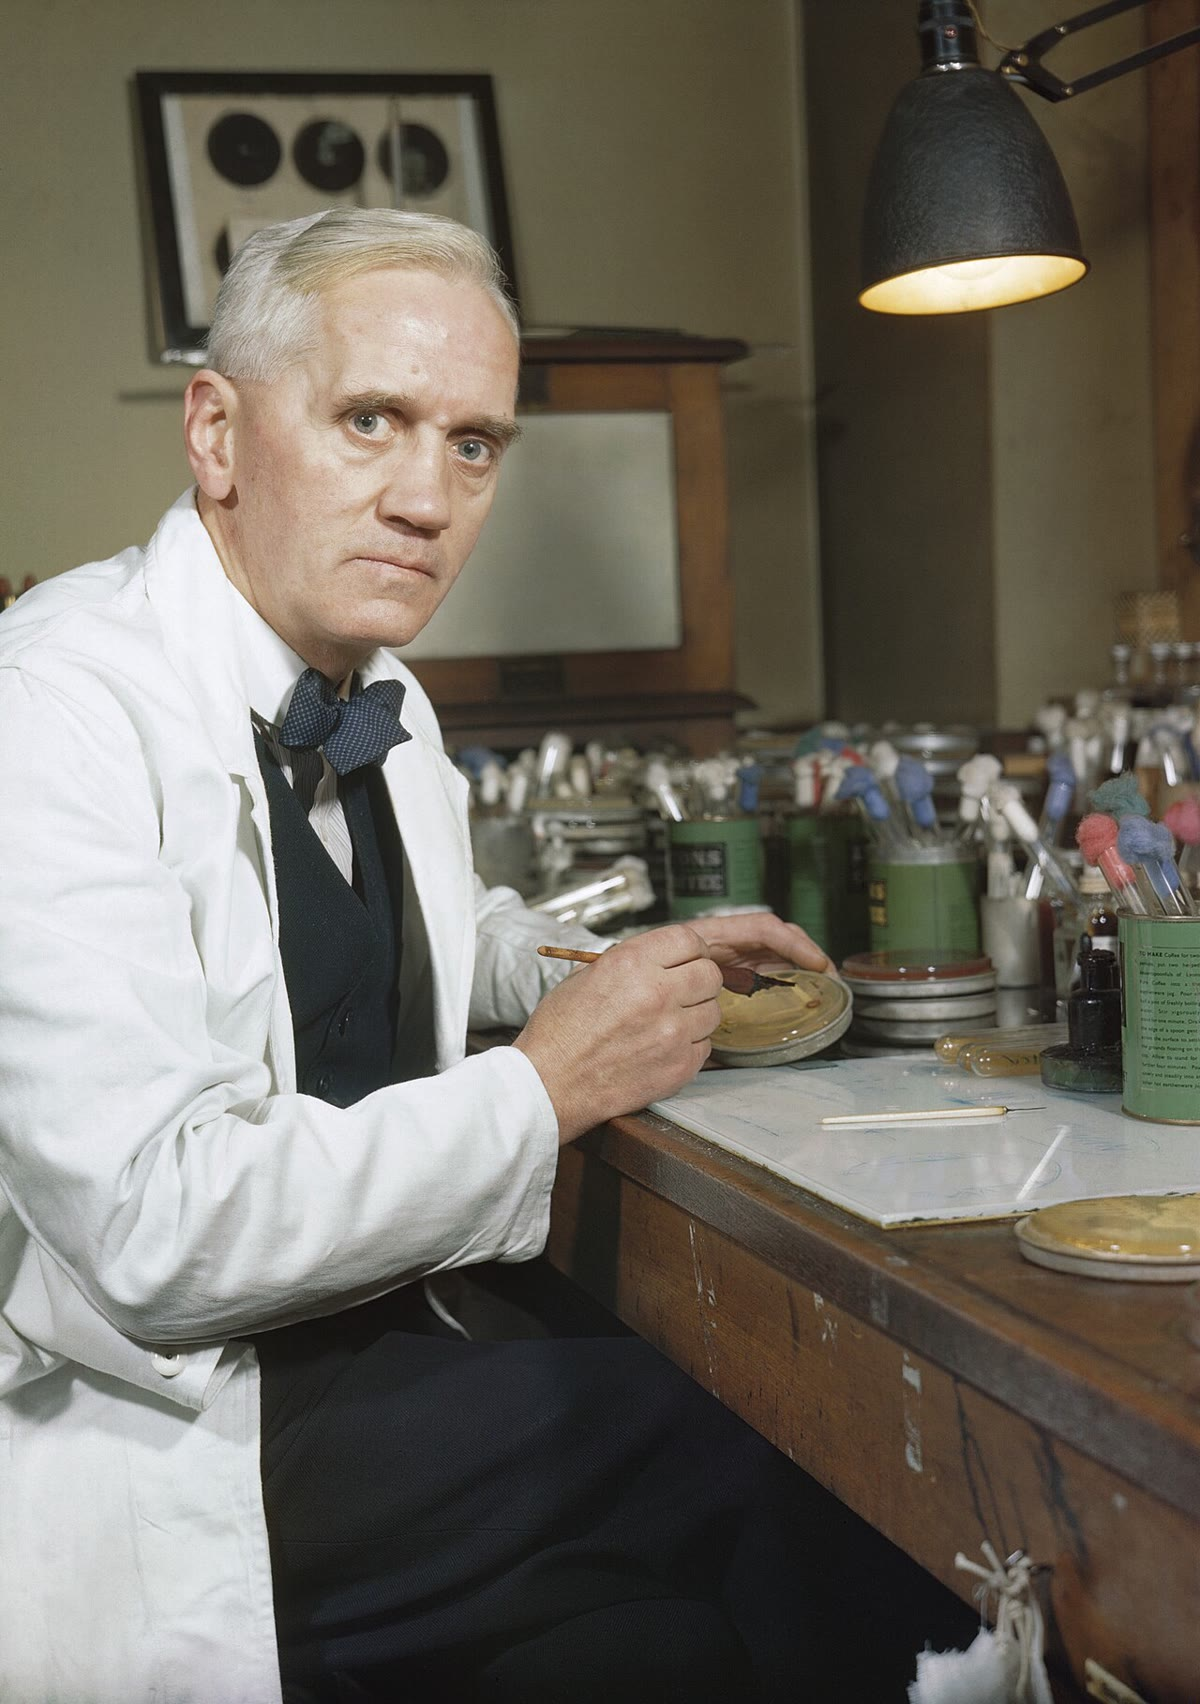
\includegraphics[width=0.4\linewidth]{images/book2/fleming.jpg}

{\small Alexander Fleming di meja kerjanya pada 1943, dengan cawan biakan yang lima belas tahun sebelumnya membuatnya memperhatikan sebuah kapang yang membersihkan bakteri di sekelilingnya. Foto, Imperial War Museums, domain publik.}
\end{omfigure}

\section{Bagaimana bakteri beragam}

\begin{proposition}[Perkembangbiakan dan keragaman bakteri]\label{prop:g11:antibiotic-resistance:variation}
Sebuah bakteri berkembang biak dengan membelah dua setelah menyalin
\omterm{def:g11:cell-cycle-mitosis:chromosome}{kromosom} tunggalnya: anaknya, selain kesalahan penyalinannya, secara
genetik serupa dengan induknya --- sebuah \emph{klon}. Dalam medium
yang kaya, satu pembelahan tiap 20 menit mengubah satu \omterm{def:g10:cells-common-unit:cell}{sel} menjadi satu
miliar dalam sepuluh jam. Keragaman genetik dalam klonnya berasal dari
dua sumber:
\begin{itemize}
  \item \emph{\omterm{def:g11:mutations:mutation}{mutasi}} (\cref{ch:g11:mutations}), yang langka tiap
        pembelahan tetapi sering pada populasi bermiliar-miliar;
  \item \emph{pemindahan gen mendatar}\index{pemindahan gen mendatar}:
        \omterm{def:g10:universal-dna:information}{DNA} yang diterima dari bakteri lain, dari \omterm{def:g10:biodiversity-scales:species}{spesies} yang sama
        atau \omterm{def:g10:biodiversity-scales:species}{spesies} lain, paling sering sebagai sebuah \emph{plasmid}
        --- lingkaran \omterm{def:g10:universal-dna:information}{DNA} kecil, yang terpisah dari \omterm{def:g11:cell-cycle-mitosis:chromosome}{kromosomnya},
        membawa beberapa \omterm{def:g10:universal-dna:gene}{gen} dan mampu berpindah dari \omterm{def:g10:cells-common-unit:cell}{sel} ke \omterm{def:g10:cells-common-unit:cell}{sel} lewat
        sebuah jembatan membran.
\end{itemize}
\end{proposition}
\admitted

\begin{omfigure}
\begin{tikzpicture}[font=\small, >=Stealth]
  % donor
  \draw[thick, fill=omDef!10, rounded corners=12pt] (0,0) rectangle (3,1.5);
  \draw[thick, omDef] (0.4,0.75) .. controls (0.6,1.3) and (2.4,1.3) .. (2.6,0.75) .. controls (2.4,0.2) and (0.6,0.2) .. (0.4,0.75);
  \draw[thick, omThm, fill=omThm!20] (2.2,1.15) circle (0.22);
  \node[anchor=north] at (1.5,-0.1) {pendonor: punya plasmidnya};
  % recipient
  \draw[thick, fill=omDef!10, rounded corners=12pt] (5,0) rectangle (8,1.5);
  \draw[thick, omDef] (5.4,0.75) .. controls (5.6,1.3) and (7.4,1.3) .. (7.6,0.75) .. controls (7.4,0.2) and (5.6,0.2) .. (5.4,0.75);
  \node[anchor=north] at (6.5,-0.1) {penerima};
  % bridge
  \draw[thick, fill=omProp!30] (3,0.55) rectangle (5,0.95);
  \draw[->, thick, omThm] (3.1,0.75) -- (4.9,0.75);
  \node[anchor=north, font=\scriptsize] at (4,-0.6) {satu salinan plasmidnya menyeberangi jembatannya};
  % result
  \draw[->, thick] (8.4,0.75) -- (9.2,0.75);
  \draw[thick, fill=omDef!10, rounded corners=12pt] (9.5,0) rectangle (12.5,1.5);
  \draw[thick, omDef] (9.9,0.75) .. controls (10.1,1.3) and (11.9,1.3) .. (12.1,0.75) .. controls (11.9,0.2) and (10.1,0.2) .. (9.9,0.75);
  \draw[thick, omThm, fill=omThm!20] (11.7,1.15) circle (0.22);
  \node[anchor=north, align=center] at (11,-0.1) {penerimanya kini membawa\\ gen plasmidnya};
  \node[anchor=west, font=\scriptsize, omDef] at (0.2,1.75) {kromosom};
  \node[anchor=west, font=\scriptsize, omThm] at (2.5,1.75) {plasmid};
\end{tikzpicture}

{\small Pemindahan mendatar. Sebuah plasmid --- lingkaran \omterm{def:g10:universal-dna:information}{DNA} kecil
yang mungkin membawa \omterm{def:g10:universal-dna:gene}{gen} ketahanan --- disalin menyeberangi sebuah
jembatan dari satu bakteri ke bakteri lain, yang tidak harus dari
\omterm{def:g10:biodiversity-scales:species}{spesies} yang sama. Penerimanya, dan seluruh keturunannya, memperoleh
\omterm{def:g10:universal-dna:gene}{gen} itu dalam satu langkah.}
\end{omfigure}

\begin{example}[Hitungan sebuah populasi]\label{ex:g11:antibiotic-resistance:arithmetic}
\omterm{def:g11:mutations:mutation}{Mutasi} ketahanan muncul sekitar sekali tiap $10^8$ pembelahan. Karena
itu sebuah labu berisi $10^9$ bakteri telah mengalami, dalam pembelahan
yang menghasilkannya, sekitar sepuluh \omterm{def:g11:mutations:mutation}{mutasi} semacam itu; luka yang
terinfeksi atau sebuah usus, dengan $10^{12}$ bakteri, sekitar sepuluh
ribu. Tiap populasi bakteri yang besar memuat, sebelum \omterm{def:g11:antibiotic-resistance:antibiotic}{antibiotik} apa
pun dipakai, \omterm{def:g10:cells-common-unit:cell}{sel} yang \omterm{prop:g11:antibiotic-resistance:mechanisms}{tahan} terhadapnya --- cawan replika
\cref{ch:g11:mutations} membuktikannya.
\end{example}

\section{Antibiotik}

\begin{definition}[Antibiotik]\label{def:g11:antibiotic-resistance:antibiotic}
Sebuah \emph{antibiotik}\index{antibiotik} adalah molekul yang membunuh
bakteri atau menghentikan pertumbuhannya, pada kepekatan yang tidak
membahayakan \omterm{def:g10:cells-common-unit:cell}{sel} pasiennya, dengan bekerja pada struktur atau proses
yang dimiliki bakteri dan tidak dimiliki \omterm{def:g10:cells-common-unit:cell}{sel} manusia: penisilin dan
kerabatnya menghalangi pembangunan dinding bakterinya; streptomisin dan
tetrasiklin menjepit \omterm{def:g10:cells-common-unit:organelle}{ribosom} bakterinya, yang berbeda dari \omterm{def:g10:cells-common-unit:organelle}{ribosom}
kita; yang lain menghalangi \omterm{def:g11:enzymes-and-phenotype:enzyme}{enzim} bakteri bagi \omterm{def:g11:dna-replication:replication}{replikasi DNA}. Sebagian
besarnya mula-mula ditemukan dalam kapang dan bakteri tanah, yang
membuatnya untuk melawan pesaingnya. Antibiotik tidak berpengaruh pada
virus, yang tidak punya satu pun sasaran itu.
\end{definition}

\begin{proposition}[Mekanisme ketahanannya]\label{prop:g11:antibiotic-resistance:mechanisms}
Sebuah bakteri bersifat \emph{tahan}\index{ketahanan antibiotik}
terhadap sebuah \omterm{def:g11:antibiotic-resistance:antibiotic}{antibiotik} ketika ia tumbuh pada kepekatan yang
menghentikan kerabatnya yang peka. Ketahanannya punya dasar genetik
dari beberapa macam: sebuah \omterm{def:g10:universal-dna:gene}{gen} bagi \omterm{def:g11:enzymes-and-phenotype:enzyme}{enzim} yang memusnahkan
\omterm{def:g11:antibiotic-resistance:antibiotic}{antibiotiknya} (penisilinase memotong penisilin menjadi dua); \omterm{def:g11:mutations:mutation}{mutasi}
yang mengubah sasaran \omterm{def:g11:antibiotic-resistance:antibiotic}{antibiotiknya} sehingga obatnya tidak lagi
mengikat (\omterm{def:g11:gene-expression:protein}{protein} \omterm{def:g10:cells-common-unit:organelle}{ribosom} yang berubah); sebuah pompa yang mengusir
obatnya; dinding yang tidak membiarkannya masuk. Masing-masing berupa
sebuah \omterm{def:g10:universal-dna:gene}{alel} atau \omterm{def:g10:universal-dna:gene}{gen}, dan masing-masing diwariskan --- secara tegak
oleh klonnya dan, jika berada pada plasmid, secara mendatar oleh
tetangganya.
\end{proposition}
\admitted

\begin{method}[Membaca sebuah antibiogram]\label{met:g11:antibiotic-resistance:antibiogram}
Sebuah \emph{antibiogram} menguji bakteri seorang pasien terhadap
beberapa \omterm{def:g11:antibiotic-resistance:antibiotic}{antibiotik} sekaligus.
\begin{enumerate}
  \item Sebarkan bakterinya merata pada sebuah cawan; letakkan cakram
        kertas yang masing-masing dibasahi satu \omterm{def:g11:antibiotic-resistance:antibiotic}{antibiotik}; eramkan
        semalam.
  \item \omterm{def:g11:antibiotic-resistance:antibiotic}{Antibiotiknya} meresap keluar dari cakramnya, kepekatannya turun
        seiring jarak; bakterinya tumbuh menjadi hamparan kecuali di
        tempat kepekatannya menghentikannya: sebuah \emph{zona hambat}
        yang bening di sekeliling tiap cakram.
  \item Ukurlah garis tengah tiap zonanya dan bandingkan dengan ambang
        yang ditetapkan bagi \omterm{def:g11:antibiotic-resistance:antibiotic}{antibiotik} itu: garis tengah di atas
        ambangnya berarti peka, di bawahnya berarti \omterm{prop:g11:antibiotic-resistance:mechanisms}{tahan}.
  \item Zona terbesar di antara hasil yang peka menuntun peresepannya;
        cakram tanpa zona sama sekali adalah \omterm{def:g11:antibiotic-resistance:antibiotic}{antibiotik} yang diabaikan
        galurnya.
\end{enumerate}
\end{method}

\begin{omfigure}
\begin{tikzpicture}[font=\small]
  \draw[thick, fill=omProp!12] (0,0) circle (3.7);
  \foreach \a/\r/\l in {90/1.3/A, 162/0.9/B, 234/0.0/C, 306/1.6/D, 18/0.55/E} {
    \begin{scope}[shift={(\a:2.0)}]
      \ifdim \r pt > 0pt \draw[fill=white] (0,0) circle (\r); \fi
      \draw[fill=gray!30] (0,0) circle (0.28);
      \node[font=\scriptsize] at (0,0) {\l};
    \end{scope}
  }
  \node[anchor=west, align=left] at (3.8,1.6) {A: zona \qty{26}{mm}, ambang 17: peka};
  \node[anchor=west, align=left] at (3.8,0.9) {B: zona \qty{18}{mm}, ambang 20: tahan};
  \node[anchor=west, align=left] at (3.8,0.2) {C: tanpa zona: tahan};
  \node[anchor=west, align=left] at (3.8,-0.5) {D: zona \qty{32}{mm}, ambang 22: peka};
  \node[anchor=west, align=left] at (3.8,-1.2) {E: zona \qty{11}{mm}, ambang 15: tahan};
  \node[anchor=north, align=center] at (0,-3.9) {hamparan bakteri pasiennya;\\ cakram agar bening yang putih di sekeliling cakram antibiotiknya};
\end{tikzpicture}

{\small Sebuah antibiogram yang terbaca. Tiap cakram memuat satu
\omterm{def:g11:antibiotic-resistance:antibiotic}{antibiotik}; zona yang bening adalah tempat bakterinya tidak dapat
tumbuh. Jika dibandingkan dengan ambang tiap obatnya, garis tengahnya
menggolongkan galurnya peka terhadap A dan D, \omterm{prop:g11:antibiotic-resistance:mechanisms}{tahan} terhadap B, C dan E.}
\end{omfigure}

\begin{omfigure}
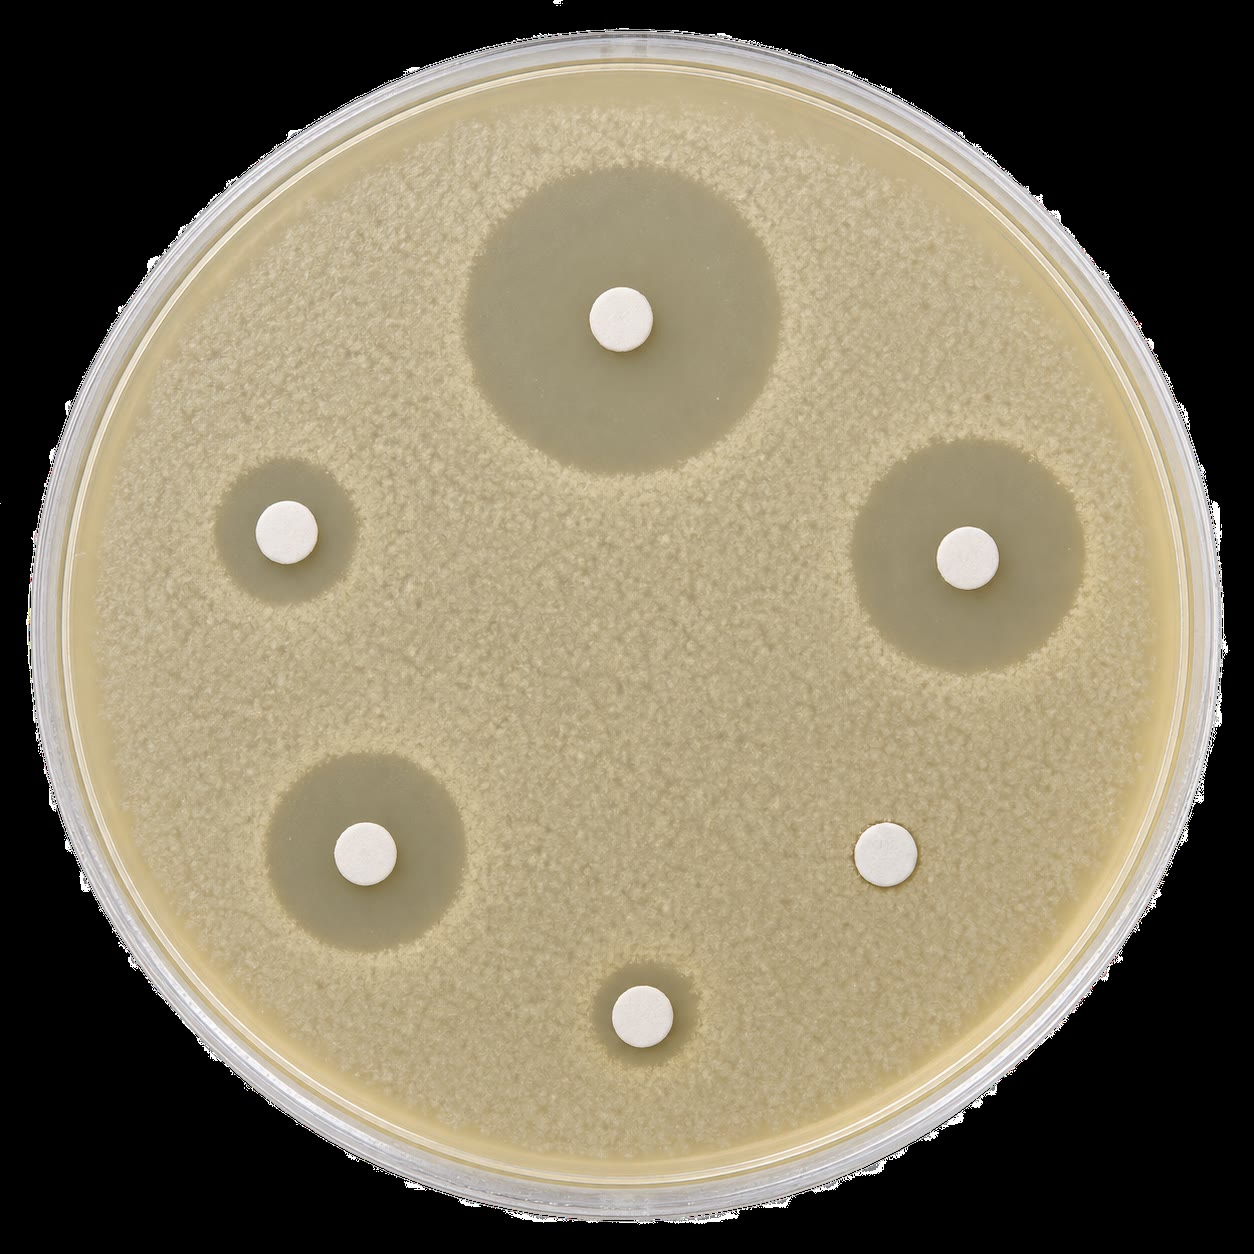
\includegraphics[width=0.44\linewidth]{images/book2/ai/g11-antibiogram-plate.jpg}

{\small Sebuah cawan antibiogram setelah pengeraman semalam: sebuah
hamparan bakteri, dan di sekeliling tiap cakram \omterm{def:g11:antibiotic-resistance:antibiotic}{antibiotiknya} sebuah
zona bening yang besarnya mengukur kepekaan galurnya. Satu cakram tanpa zona.}
\end{omfigure}

\section{Bagaimana ketahanannya menyebar}

\begin{proposition}[Seleksi oleh antibiotiknya]\label{prop:g11:antibiotic-resistance:selection}
Sebuah \omterm{def:g11:antibiotic-resistance:antibiotic}{antibiotik} tidak menciptakan bakteri yang \omterm{prop:g11:antibiotic-resistance:mechanisms}{tahan}; ia
\emph{memilih}-nya. Dalam populasi yang beberapa \omterm{def:g10:cells-common-unit:cell}{selnya} membawa \omterm{def:g10:universal-dna:gene}{alel}
ketahanan, obatnya membunuh atau menghentikan mayoritas yang peka dan
membiarkan segelintir yang \omterm{prop:g11:antibiotic-resistance:mechanisms}{tahan} berlipat ganda tanpa persaingan: dalam
beberapa hari populasinya menjadi \omterm{prop:g11:antibiotic-resistance:mechanisms}{tahan}. Makin banyak sebuah \omterm{def:g11:antibiotic-resistance:antibiotic}{antibiotik}
dipakai --- pada pasien, pada hewan, di lingkungan --- makin sering
pemilahan ini terjadi, dan makin \omterm{prop:g11:antibiotic-resistance:mechanisms}{tahan} bakteri sebuah rumah sakit,
peternakan atau negeri. Rangkaian yang tidak lengkap, yang membunuh \omterm{def:g10:cells-common-unit:cell}{sel}
yang paling peka dan menyayangi yang paling tidak peka, memilih paling
tepat guna di antara semuanya.
\end{proposition}
\begin{proof}[Bukti percobaan]
Cawan replika Lederberg menunjukkan \omterm{def:g10:cells-common-unit:cell}{sel} yang \omterm{prop:g11:antibiotic-resistance:mechanisms}{tahan} sudah hadir sebelum
paparannya. Biakan yang ditumbuhkan sepekan dalam kepekatan \omterm{def:g11:antibiotic-resistance:antibiotic}{antibiotik}
yang meningkat berakhir \omterm{prop:g11:antibiotic-resistance:mechanisms}{tahan} terhadap seratus kali dosis awalnya, dan
ketahanannya diwariskan serta terpetakan pada \omterm{def:g11:mutations:mutation}{mutasi} tertentu. Negeri
yang paling banyak memakai \omterm{def:g11:antibiotic-resistance:antibiotic}{antibiotik} tiap orang punya bagian galur
yang \omterm{prop:g11:antibiotic-resistance:mechanisms}{tahan} paling tinggi; bangsal rumah sakit yang mengurangi
pemakaiannya melihat ketahanannya turun sepanjang beberapa bulan.
Sebuah galur bakteri kulit \emph{Staphylococcus aureus} yang \omterm{prop:g11:antibiotic-resistance:mechanisms}{tahan}
terhadap penisilin muncul dalam empat tahun setelah obatnya
diperkenalkan dan kini menjelaskan sebagian besar galur rumah sakit;
galur yang \omterm{prop:g11:antibiotic-resistance:mechanisms}{tahan} terhadap obat penggantinya menyusul penggantinya dalam
dua tahun.
\end{proof}

\begin{omfigure}
\begin{tikzpicture}
\begin{axis}[
  width=0.88\linewidth, height=5.8cm,
  axis x line=bottom, axis y line=left,
  xmin=0, xmax=6, ymin=0, ymax=110,
  xlabel={hari pengobatan}, ylabel={bakteri (\% dari awalnya)},
  xlabel style={font=\small, at={(axis description cs:0.5,-0.12)}, anchor=north},
  ylabel style={font=\small},
  tick label style={font=\small}, xtick={0,1,2,3,4,5,6}, ytick={0,25,50,75,100},
  legend style={at={(0.5,-0.3)}, anchor=north, legend columns=3, font=\small, draw=none},
  clip=false,
]
\addplot[thick, omDef] coordinates {(0,100) (0.5,45) (1,15) (1.5,5) (2,1.5) (3,0.2) (4,0.05) (5,0.01) (6,0)};
\addplot[thick, omThm] coordinates {(0,0.001) (1,0.01) (2,0.1) (3,1) (4,8) (5,40) (6,100)};
\addplot[thick, omMeth, dashed] coordinates {(0,100) (0.5,45) (1,15) (1.5,5) (2,1.5) (3,1.2) (4,9) (5,48) (6,100)};
\legend{sel peka, sel tahan (satu tiap $10^5$), seluruhnya jika pengobatan berhenti hari ke-3}
\end{axis}
\end{tikzpicture}

{\small Seleksi selama satu rangkaian \omterm{def:g11:antibiotic-resistance:antibiotic}{antibiotik}. \omterm{def:g10:cells-common-unit:cell}{Sel} yang peka (biru)
terbunuh dalam beberapa hari; segelintir yang \omterm{prop:g11:antibiotic-resistance:mechanisms}{tahan} (merah) berlipat
ganda tanpa lawan dan, pada akhir pekannya, menyusun seluruh
populasinya. Jika pasiennya berhenti pada hari ke-3, yang selamat
tumbuh kembali --- kini hampir seluruhnya \omterm{prop:g11:antibiotic-resistance:mechanisms}{tahan}.}
\end{omfigure}

\begin{example}[Dari satu sel ke sebuah bangsal]\label{ex:g11:antibiotic-resistance:ward}
Seorang pasien yang diobati dengan penisilin membawa, di antara
$10^{10}$ bakteri, seratus bakteri yang \omterm{prop:g11:antibiotic-resistance:mechanisms}{tahan}. Dalam tiga hari yang
peka telah lenyap dan klon yang \omterm{prop:g11:antibiotic-resistance:mechanisms}{tahan} telah mengambil tempatnya:
$10^{10}$ \omterm{def:g10:cells-common-unit:cell}{sel} yang \omterm{prop:g11:antibiotic-resistance:mechanisms}{tahan}. Di tangan seorang perawat, pada pegangan
tempat tidur, dalam tubuh pasien berikutnya, klonnya berlanjut --- dan
jika \omterm{def:g10:universal-dna:gene}{gen} ketahanannya berada pada sebuah plasmid, ia menyerahkannya
kepada \omterm{def:g10:biodiversity-scales:species}{spesies} lain di sepanjang jalannya. Tidak ada satu pun dalam
runtunan ini yang menuntut \omterm{def:g11:antibiotic-resistance:antibiotic}{antibiotiknya} bekerja pada \omterm{def:g10:universal-dna:information}{DNA}; ia hanya
menyingkirkan persaingannya.
\end{example}

\section{Menjaga antibiotik tetap bekerja}

\begin{proposition}[Akibat dan tanggapannya]\label{prop:g11:antibiotic-resistance:consequences}
Infeksi yang \omterm{prop:g11:antibiotic-resistance:mechanisms}{tahan} berlangsung lebih lama, lebih mahal dan lebih sering
mematikan; sebagian galur kini menahan setiap obat yang tersedia.
Karena ketahanannya digerakkan pemakaiannya, tanggapannya adalah
memakai \omterm{def:g11:antibiotic-resistance:antibiotic}{antibiotik} lebih sedikit dan lebih baik: hanya bagi infeksi
bakteri (tidak pernah bagi pilek dan flu virus), yang dipilih setelah
antibiogram bila mungkin, pada dosis penuh selama rangkaian yang penuh,
dengan obat tersempit yang berhasil; membatasi pemakaiannya dalam
pertanian; mencegah infeksi (kebersihan, vaksinasi) sehingga rangkaian
yang diperlukan lebih sedikit; dan mengasingkan \omterm{def:g11:genes-and-disease:genetic}{pembawa} galur yang
\omterm{prop:g11:antibiotic-resistance:mechanisms}{tahan} di rumah sakit. \omterm{def:g11:antibiotic-resistance:antibiotic}{Antibiotik} baru membeli waktu; hitungan
seleksinya menjamin bahwa ketahanan terhadap masing-masingnya akan muncul.
\end{proposition}
\admitted

\begin{remark}[Evolusi dalam sepekan]\label{rem:g11:antibiotic-resistance:evolution}
\omterm{def:g11:mutations:mutation}{Mutasi} memasok keragaman secara acak, lingkungannya memilahnya,
keturunan yang selamat mewarisi bedanya: bakteri bab ini menjalankan,
dalam sepekan, proses yang akan dilukiskan tahun terakhir sepanjang
jutaan tahun bagi paus dan pohon ek. Ketahanan terhadap \omterm{def:g11:antibiotic-resistance:antibiotic}{antibiotik}
adalah evolusi lewat seleksi alam yang teramati secara langsung, dengan
manusia sebagai pemilahnya --- dan menjadi peragaan yang paling jernih
bahwa prosesnya bukan teori tentang masa lalu melainkan kenyataan
tentang populasi mana pun yang beragam dan berkembang biak.
\end{remark}

\section{Latihan}

\begin{exercise}[$\star$]\label{exo:g11:antibiotic-resistance:1}
Sebutkan kedua sumber keragaman genetik dalam sebuah populasi bakteri.
\end{exercise}

\begin{exercise}[$\star$]\label{exo:g11:antibiotic-resistance:2}
Apa itu \omterm{def:g11:antibiotic-resistance:antibiotic}{antibiotik}, dan mengapa ia membahayakan bakteri tetapi tidak
\omterm{def:g10:cells-common-unit:cell}{sel} pasiennya? Mengapa ia tidak berguna melawan pilek?
\end{exercise}

\begin{exercise}[$\star$]\label{exo:g11:antibiotic-resistance:3}
Berikan tiga mekanisme yang dengannya bakteri dapat menahan \omterm{def:g11:antibiotic-resistance:antibiotic}{antibiotik}.
\end{exercise}

\begin{exercise}[$\star$]\label{exo:g11:antibiotic-resistance:4}
Pada gambar antibiogramnya, cakram baru F memberi zona
\qty{20}{mm} dengan ambang \qty{18}{mm}. Peka atau \omterm{prop:g11:antibiotic-resistance:mechanisms}{tahan}? \omterm{def:g11:antibiotic-resistance:antibiotic}{Antibiotik}
mana yang akan kamu resepkan di antara A sampai F?
\end{exercise}

\begin{exercise}[$\star$]\label{exo:g11:antibiotic-resistance:5}
Apakah sebuah \omterm{def:g11:antibiotic-resistance:antibiotic}{antibiotik} menyebabkan \omterm{def:g11:mutations:mutation}{mutasi} ketahanan? Berikan
alasannya dengan percobaan \cref{ch:g11:mutations}.
\end{exercise}

\begin{exercise}[$\star\star$]\label{exo:g11:antibiotic-resistance:6}
Mulai dari satu bakteri yang membelah tiap 20 menit, ada berapa bakteri
setelah 10 jam? Jika ketahanannya muncul sekali tiap $10^8$ pembelahan,
berapa \omterm{def:g10:cells-common-unit:cell}{sel} \omterm{prop:g11:antibiotic-resistance:mechanisms}{tahan} yang mungkin dimuat biakannya?
\end{exercise}

\begin{exercise}[$\star\star$]\label{exo:g11:antibiotic-resistance:7}
Dari gambar seleksinya, pada hari keberapa \omterm{def:g10:cells-common-unit:cell}{sel} yang \omterm{prop:g11:antibiotic-resistance:mechanisms}{tahan} menjadi
mayoritas seluruhnya? Berapa populasi seluruhnya pada hari ke-6 pada
hal yang bergaris putus-putus, dan ia tersusun dari apa?
\end{exercise}

\begin{exercise}[$\star\star$]\label{exo:g11:antibiotic-resistance:8}
Jelaskan mengapa \omterm{def:g10:universal-dna:gene}{gen} ketahanan pada sebuah plasmid menyebar lebih cepat
daripada \omterm{def:g10:universal-dna:gene}{gen} pada \omterm{def:g11:cell-cycle-mitosis:chromosome}{kromosomnya}.
\end{exercise}

\begin{exercise}[$\star\star$]\label{exo:g11:antibiotic-resistance:9}
Seorang pasien merasa lebih baik setelah tiga hari dari rangkaian tujuh
hari lalu berhenti. Jelaskan, dengan gambarnya, apa yang terjadi pada
hari-hari berikutnya dan mengapa kambuhnya lebih sulit diobati.
\end{exercise}

\begin{exercise}[$\star\star$]\label{exo:g11:antibiotic-resistance:10}
Mengapa bagian galur yang \omterm{prop:g11:antibiotic-resistance:mechanisms}{tahan} lebih tinggi di rumah sakit daripada
pada populasi umum?
\end{exercise}

\begin{exercise}[$\star\star$]\label{exo:g11:antibiotic-resistance:11}
Jelaskan mengapa \omterm{def:g11:mutations:mutation}{mutasi} yang mengubah \omterm{def:g11:gene-expression:protein}{protein} \omterm{def:g10:cells-common-unit:organelle}{ribosom} dapat membuat
bakteri \omterm{prop:g11:antibiotic-resistance:mechanisms}{tahan} terhadap streptomisin, dan mengapa bakteri semacam itu
sering tumbuh sedikit lebih lambat daripada kerabatnya yang peka.
\end{exercise}

\begin{exercise}[$\star\star\star$]\label{exo:g11:antibiotic-resistance:12}
Dua \omterm{def:g11:antibiotic-resistance:antibiotic}{antibiotik} dengan sasaran yang berbeda diberikan bersama.
Perkirakan peluang sebuah \omterm{def:g10:cells-common-unit:cell}{sel} \omterm{prop:g11:antibiotic-resistance:mechanisms}{tahan} terhadap keduanya lewat \omterm{def:g11:mutations:mutation}{mutasi} yang
saling bebas (satu tiap $10^8$ masing-masing), dan jelaskan mengapa
terapi gabungan dipakai melawan infeksi yang lambat dan panjang seperti
tuberkulosis.
\end{exercise}

\begin{exercise}[$\star\star\star$]\label{exo:g11:antibiotic-resistance:13}
Sebuah peternakan menambahkan \omterm{def:g11:antibiotic-resistance:antibiotic}{antibiotik} dosis rendah ke pakan
ternaknya untuk mempercepat pertumbuhan. Ramalkan akibatnya bagi
bakteri ternaknya, bagi pekerja peternakannya, dan bagi kedokteran
manusia, dengan memakai seleksi dan pemindahan mendatarnya.
\end{exercise}

\begin{exercise}[$\star\star\star$]\label{exo:g11:antibiotic-resistance:14}
Sebuah bangsal membagi dua peresepan \omterm{def:g11:antibiotic-resistance:antibiotic}{antibiotiknya}; dalam setahun
bagian galur yang \omterm{prop:g11:antibiotic-resistance:mechanisms}{tahan} turun. Jelaskan mengapa ketahanannya dapat
surut, dengan memakai harga ketahanan bagi bakterinya dan persaingannya.
\end{exercise}

\begin{exercise}[$\star\star\star$]\label{exo:g11:antibiotic-resistance:15}
``Bakteri menjadi \omterm{prop:g11:antibiotic-resistance:mechanisms}{tahan} karena ia terbiasa dengan \omterm{def:g11:antibiotic-resistance:antibiotic}{antibiotiknya}.''
Tuliskan ulang kalimat ini dengan benar, dalam satu paragraf pendek,
dengan memakai \omterm{def:g11:mutations:mutation}{mutasi}, seleksi dan pewarisannya.
\end{exercise}

\section{Soal: Bangsalnya}

\begin{problem}[{Soal akhir pekan --- sebuah wabah di bangsal rumah
sakit yang diikuti dari satu sel mutan: hitungan sebuah koloni, sebuah
antibiogram yang terbaca, satu rangkaian yang terputus, dan kebijakan
yang menghentikan penyebarannya}]
\label{pb:g11:antibiotic-resistance:1}
Luka seorang pasien terinfeksi $10^{10}$ bakteri dari satu \omterm{def:g10:biodiversity-scales:species}{spesies}.
Bakterinya membelah tiap 30 menit; \omterm{def:g11:mutations:mutation}{mutasi} yang memberi ketahanan
terhadap \omterm{def:g11:antibiotic-resistance:antibiotic}{antibiotik} amoksisilin terjadi sekali tiap $10^8$ pembelahan.
\omterm{def:g11:antibiotic-resistance:antibiotic}{Antibiotiknya} membunuh 90\% \omterm{def:g10:cells-common-unit:cell}{sel} yang peka tiap 6 jam dan tidak
mempengaruhi \omterm{def:g10:cells-common-unit:cell}{sel} yang \omterm{prop:g11:antibiotic-resistance:mechanisms}{tahan}, yang terus membelah.

\medskip
\noindent\textbf{Bagian I --- Sebelum pengobatannya.}
\begin{enumerate}
  \item Berapa pembelahan yang menghasilkan $10^{10}$ bakteri itu dari
        \omterm{def:g10:cells-common-unit:cell}{sel} pertamanya? (Hitunglah jumlah \omterm{def:g10:cells-common-unit:cell}{selnya}.)
  \item Perkirakan jumlah \omterm{def:g10:cells-common-unit:cell}{sel} yang \omterm{prop:g11:antibiotic-resistance:mechanisms}{tahan} yang hadir sebelum \omterm{def:g11:antibiotic-resistance:antibiotic}{antibiotik}
        apa pun diberikan.
  \item Jelaskan mengapa infeksi pasiennya tetap dilukiskan sebagai
        ``peka'' pada antibiogramnya.
  \item Antibiogramnya memperlihatkan zona \qty{24}{mm} bagi
        amoksisilin (ambang 17), \qty{12}{mm} bagi eritromisin (ambang
        20) dan tanpa zona bagi penisilin. Tafsirkan ketiga hasilnya.
  \item Dokternya meresepkan amoksisilin selama 7 hari. Mengapa bukan
        penisilin, dan mengapa bukan obat dengan zona terbesar
        seandainya ada yang lebih besar?
\end{enumerate}

\medskip
\noindent\textbf{Bagian II --- Selama pengobatannya.}
\begin{enumerate}[resume]
  \item Berapa \omterm{def:g10:cells-common-unit:cell}{sel} peka yang tersisa setelah 1 hari? Setelah 3 hari?
  \item Mulai dari jawabanmu atas pertanyaan 2, berapa \omterm{def:g10:cells-common-unit:cell}{sel} yang \omterm{prop:g11:antibiotic-resistance:mechanisms}{tahan}
        setelah 1 hari jika \omterm{def:g10:cells-common-unit:cell}{sel} itu berlipat dua tiap 30 menit tanpa
        batas? (Pakai $2^{48} \approx \num{2.8e14}$.) Mengapa angka ini
        tidak masuk akal, dan apa yang membatasinya?
  \item Andaikan klon yang \omterm{prop:g11:antibiotic-resistance:mechanisms}{tahan} itu terbatas pada ruang yang
        dikosongkan \omterm{def:g10:cells-common-unit:cell}{sel} yang peka, sehingga ia tidak dapat melampaui
        $10^{10}$. Kira-kira kapan ia mengisi ruang itu?
  \item Sketsakan, atau lukiskan, lengkung \omterm{def:g10:cells-common-unit:cell}{sel} yang peka, \omterm{def:g10:cells-common-unit:cell}{sel} yang
        \omterm{prop:g11:antibiotic-resistance:mechanisms}{tahan} dan seluruh \omterm{def:g10:cells-common-unit:cell}{selnya} sepanjang 7 hari itu.
  \item Sesungguhnya sistem kekebalan pasiennya membersihkan beberapa
        juta \omterm{def:g10:cells-common-unit:cell}{sel} terakhir dari jenis mana pun dalam beberapa hari.
        Jelaskan mengapa hasilnya bergantung pada apakah klon yang
        \omterm{prop:g11:antibiotic-resistance:mechanisms}{tahan} tumbuh lebih cepat daripada pembersihan oleh sistem
        kekebalannya.
\end{enumerate}

\medskip
\noindent\textbf{Bagian III --- Rangkaian yang terputus.}
\begin{enumerate}[resume]
  \item Pasiennya berhenti setelah 2 hari, karena merasa sehat. Berapa
        \omterm{def:g10:cells-common-unit:cell}{sel} peka yang tersisa, dan berapa bagian populasi yang selamat
        yang bersifat \omterm{prop:g11:antibiotic-resistance:mechanisms}{tahan}?
  \item Bakterinya tumbuh kembali menjadi $10^{10}$ pada hari-hari
        berikutnya. Berapa bagiannya yang kini \omterm{prop:g11:antibiotic-resistance:mechanisms}{tahan}, jika \omterm{def:g10:cells-common-unit:cell}{sel} yang
        \omterm{prop:g11:antibiotic-resistance:mechanisms}{tahan} dan \omterm{def:g10:cells-common-unit:cell}{sel} yang peka tumbuh dengan laju yang sama?
  \item Pasiennya kambuh dan diberi amoksisilin lagi. Ramalkan hasilnya.
  \item Antibiogram kambuhnya tidak memperlihatkan zona bagi
        amoksisilin. Jelaskan perubahannya dari antibiogram yang pertama.
  \item \omterm{def:g10:universal-dna:gene}{Gen} ketahanannya berada pada sebuah plasmid. Risiko apa lagi
        yang ditambahkannya bagi bangsalnya?
\end{enumerate}

\medskip
\noindent\textbf{Bagian IV --- Kebijakan bangsalnya.}
Bangsalnya mengobati 400 pasien tiap tahun dengan amoksisilin; 30\%
infeksi yang terpencilkan di bangsalnya kini \omterm{prop:g11:antibiotic-resistance:mechanisms}{tahan}, berhadapan dengan
5\% di kotanya.
\begin{enumerate}[resume]
  \item Jelaskan beda antara bangsalnya dan kotanya dalam istilah
        tekanan seleksinya.
  \item Bangsalnya memutuskan: antibiogram sebelum tiap peresepan,
        rangkaian yang penuh, kebersihan tangan, dan pengasingan
        \omterm{def:g11:genes-and-disease:genetic}{pembawa} galur yang \omterm{prop:g11:antibiotic-resistance:mechanisms}{tahan}. Sebutkan mekanisme bab ini mana yang
        dikenai tiap tindakannya.
  \item Setelah dua tahun ketahanan di bangsalnya 12\%. Jelaskan
        mengapa ketahanannya turun, dan mengapa ia tidak kembali ke 5\%.
  \item Mengapa \omterm{def:g11:antibiotic-resistance:antibiotic}{antibiotik} baru, yang diperkenalkan di bangsalnya,
        tidak akan memecahkan persoalannya lebih dari beberapa tahun?
  \item Nyatakan hasilnya: jumlah \omterm{def:g10:cells-common-unit:cell}{sel} \omterm{prop:g11:antibiotic-resistance:mechanisms}{tahan} yang dimuat lukanya sebelum
        obat apa pun, hari ketika \omterm{def:g10:cells-common-unit:cell}{sel} itu mewarisinya, dan satu
        kebiasaan pasiennya yang mengubah infeksi yang dapat
        disembuhkan menjadi sebuah wabah.
\end{enumerate}
\end{problem}
